\documentclass[smallextended]{svjour3}
\usepackage[utf8]{inputenc}
\usepackage{amsmath}%
\usepackage{amsfonts}%
\usepackage{amssymb}%
\usepackage{graphicx}
\usepackage[table, svgnames, dvipsnames]{xcolor}
\usepackage[colorinlistoftodos,
    prependcaption,
    textsize=tiny]{todonotes}
\usepackage{proba}
\usepackage{enumerate}
\usepackage{booktabs}
\usepackage{latexsym}
\usepackage{xargs}
\usepackage{mathptmx}
\usepackage{csquotes}
\usepackage{paralist}
\usepackage[numbers,sort&compress]{natbib}
\usepackage{varioref}
\usepackage[%           % Fine in most cases
            pdfpagelabels,hypertexnames=true,
            plainpages=false,
            naturalnames=false]{hyperref}
\usepackage{color}
\usepackage{booktabs}
\usepackage{siunitx}
\usepackage[section]{placeins}
\definecolor{darkblue}{rgb}{0,0.1,0.5}
\hypersetup{colorlinks,
            linkcolor=darkblue,
            anchorcolor=darkblue,
            citecolor=darkblue}
%
\DeclareMathOperator{\trace}{trace}
%
%\let\cl@chapter\undefined
%\makeatletter
%\usepackage[nameinlink, noabbrev]{cleveref}
\newcommandx{\unsure}[2][1=]{%
	\todo[%
        linecolor=gray,
        backgroundcolor=gray!25,
       bordercolor=gray, 
        #1]{#2}
}
\newcommandx{\change}[2][1=]{%
    \todo[
        linecolor=blue,
        backgroundcolor=blue!25,
        bordercolor=blue, #1]{#2}
}
\newcommandx{\info}[2][1=]{%
    \todo[
        linecolor=OliveGreen,
        backgroundcolor=OliveGreen!25,
        bordercolor=OliveGreen, #1]{#2}
}
\newcommandx{\improvement}[2][1=]{
    \todo[linecolor=FireBrick,
        backgroundcolor=FireBrick!25,
        bordercolor=FireBrick,#1]{#2}
}
\newcommandx{\thiswillnotshow}[2][1=]{\todo[disable,#1]{#2}}
%-------------------------------------------
\smartqed 
\begin{document}
	\title{%
		Threshold behavior of a stochstic vector plant model.
	}
	\subtitle{%
		The Tomato Yellow Curl Virus
	}
	\author{%
		Gabriel A. Salcedo-Varela  \and 
		Saul Diaz-Infante\thanks{Corresponding author.}
	}
	\institute{
		Gabriel Salcedo-Varela \at
		Universidad de Sonora,
		Departamento de Matem\'aticas, 
		Boulevard Luis Encinas y Rosales s/n Col. 
		Centro, Hermosillo, Sonora, CP 83000
		Hermosillo, Sonora 
		\\
        Tel.: +521 (662)-259-2155, ext. 2394
        \\
        Fax: +521 (662) 259-2219
        \\
        \email{correo@institucional}           
        \and Saul Diaz Infante Velasco 
        \at
        CONACYT-Universidad de Soonora,
		Departamento de Matem\'aticas, 
		Boulevard Luis Encinas y Rosales s/n Col. 
		Centro, Hermosillo, Sonora, CP 83000
		Hermosillo, Sonora 
		\\
        Tel.: +521 (662)-259-2155
        \\
        Fax: +521 (662) 259-2219
        \\
        \email{saul.diazinfante@unison.mx}
	}
	\date{Received: \today / Accepted: date}
	\titlerunning{SDE-vector plant}
	\authorrunning{G. Salcedo-Varela, S. Diaz-Infante}
	\maketitle
	\keywords{Keywords}
	%
	\begin{abstract}
		BACKGROUND
		\\
		PROBLEM SETUP
		\\
		FINDINGS 
		\\
		IMPLICATIONS
	\end{abstract}
	\section{Introduction}
	\improvement{Review the structure}
	\section{Deterministic base dynamics}
		\label{sec:model_formulation}
		%!TEX root = ../main.tex
\begin{equation} 
	\label{system_1} 
	\begin{aligned} 
		\dot{S_p} &= 
			-\beta_p S_p
			\frac{I_v}{N_v} + \tilde{r_1} L_p + \tilde{r_2} I_p  
		\\ 
		\dot{L_p} &= 
			\beta_p S_p
			\frac{I_v}{N_v} - b L_p - \tilde{r_1} L_p  
		\\ 
		\dot{I_p} &= 
			b L_p - \tilde{r_2} I_p  \\ 
		\dot{S_v} &= 
			-\beta_v S_v 
			\frac{I_p}{N_p} - \tilde{\gamma} S_v
			+(1-\theta) \mu  
		\\ 
		\dot{I_v} &= 
			\beta_v S_v \frac{I_p}{N_p} 
			- \tilde{\gamma} I_v
			+ \theta \mu 
	\end{aligned} 
\end{equation} 
\todo{Make a table for description of  all parameters}
\todo{Redact this conservation law to the entire system \eqref{system_1}.
Write a introductory paragraph to Thm 1}

\begin{theorem}\label{theorem_1}
	With the notation of ODE \eqref{system_1}, let
	\begin{equation*}
		\begin{aligned}
			N_v(t) &:= S_v(t) + I_v(t) 
		 	\\
		 	N_v^{\infty} &:= \frac{\mu}{\gamma}.
		 \end{aligned}
	\end{equation*}
	Then for any initial condition 
	$
		(S_p(0), L_p(0), I_p(0), S_v(0), I_v(0) )^\top
	 	\in {(0,\infty) \times (0, N^\infty_v)}
	$, she plant and vector total populations respectively satisfies
	\begin{equation*}
		\begin{aligned}
			& \frac{d N_p}{dt} =
				\frac{d}{dt}(S_p + L_p + I_p) = 0,
			\\
			& \lim_{t\to \infty}
				N_v(t) = N_v^{\infty}.
		\end{aligned}
	\end{equation*}
\end{theorem}
		\subsection{Deterministic fixed points}
			%!TEX root = ../main.tex
\todo{Fix notation to distinguish between free disease and endemic}
Here we compute the determinsitic fixed points of system 
\eqref{system_1} and show that its unicity. Thus by definition of we solve 
%
\begin{equation}
	\begin{aligned}
		-\beta_p S_p^* \frac{I_v^*}{N_v} + r(N_p-S_p^*) &= 0\\
		\beta_p S_p^* \frac{I_v^*}{N_v} - b L_p^* - r L_p^* &= 0\\
		b L_p^* - r I_p^* &= 0\\
		-\beta_v S_v^* \frac{I_p^*}{N_p} -\gamma S_v^* +(1-\theta) \mu &= 0\\
		\beta_v S_v^* \frac{I_p^*}{N_p} -\gamma I_v^* + \theta \mu &= 0.
	\end{aligned}
\end{equation}
to determine our fixed points.
%
There is two fixed points\textemdash free disease equilibrium and the 
endemic equilibrium. We characterize the fist the relation
$ L^*_p=I_p^*=I_v^*=0$, wich implies that
%
\begin{equation*}
	r(N_p-S^*_p) = 0,
\end{equation*}
%
and therefore, we obtain $S_p^*=N_p$.F or the vector population we have by 
Theorem \eqref{theorem_1} that $S_v^*+I_v^* \rightarrow \frac{\mu}{\gamma}$ as 
$\rightarrow \infty$, then $S_v^* \rightarrow \frac{\mu}{\gamma}$ when we have 
$I^*_v=0$.
%
The free disease equilibrium point is $(N_p,0,0,\frac{\mu}{\gamma},0)^{\top}$. 
For the case of endemic equilibrium point, we need suppose that $L_p^*,I_p^*,I_
v^*\neq0$ and solve each right hand side of system \eqref{system_1} in terms 
of other variable.
%
From $\dot{S_p}$, we can obtain
%
\begin{equation*}
	S^*_p= \frac{rN_{{p}}N_{{v}}}{rN_{{v}}+I^*_v\beta_{{p}}},
\end{equation*}
%
 and similar for the other equations we obtain
\begin{equation*}
	L^*_p = \frac{\beta_{{p}}S_p^* I_v^*}{N_{{v}} \left( b+r \right)},
\end{equation*}
%
\begin{equation*}
	I^*_p =\frac{b L^*_p}{r},
\end{equation*}
%
\begin{equation*}
	S^*_v =
		\frac{
			\left( 
				1-\theta 
			\right) 
			\mu\, N_{p}
		}{
			\gamma\, N_{p} + I ^ * _ p
			\beta_{v}
		},
\end{equation*}
%
Expresing the above coordinate in terms of $I_v$, we obtain
%
\improvement{rewrite as align}
\begin{equation*}
	S^*_p = 
		\frac{
			r N_p N_v
		}{
			r N_v + 
			I ^ *_v 
			\beta_p
		},
\end{equation*}
%
%
\begin{equation*}
	L ^ *_p = 
		\frac{
			\beta_p rN_p I _ v ^ *
		}{
			\left( 
				b + r 
			\right)
			(
				r N_v + I_v ^ * 
				\beta_p
			)
		},
\end{equation*}
%
%
\begin{equation*}
	I ^*_p =
		\frac{
			b \beta_p N_p I_v ^ *
		}{
			 \left(
			 	 b + r 
			 \right)
			 ( r N_v + 
			 	I_v ^ * \beta_p
			 )
		},
\end{equation*}
%
%
\begin{equation*}
	S ^ *_v =
		\frac{
			 \left( 
			 	1 - \theta 
			 \right)
			 \mu(b + r)
			 (rN_v + \beta_p I_v^*)
		}{
			\gamma(b + r)
			(r N_v + \beta_p I^*_v) + 
			b \beta_p \beta_v I_v^*
		},
\end{equation*}
%
%
We only need substituting the above expression into the differential equation 
of $I_v$ and solve the following quadratic equation
%
\begin{equation*}
	\begin{aligned}
			&
			-N_p( 
				b \gamma^2 r I^*_v N_v + 
				b \gamma^2 (I ^*_v)^2 \beta_p -
				b \gamma \mu r \theta N_v - 
				b \gamma \mu \theta I ^ *_v \beta_p + 
				b \gamma (I^*_v)^2 \beta_p \beta_v + 
				b \mu \theta I ^ *_v \beta_p ^ 2
			\\
			&-
				b \mu \theta I ^ *_v \beta_p \beta_v +
				\gamma ^ 2 r ^ 2 I ^ *_v N_v +
				\gamma ^ 2 r (I ^ *_v) ^ 2 \beta_p - 
				\gamma\mu r^2 \theta N_v - 
				\gamma\mu r \theta I^*_v 
				\beta_p - b\mu I^*_v \beta_p^2) = 0
	\end{aligned}
\end{equation*}
% 
In sake of clearnes we define 
\begin{align*}
	a_1 &:= b \gamma^2 \beta_p+b \gamma \beta_p\beta_v+\gamma^2 r \beta_p,\\
	a_2 &:=-b\gamma\mu\theta\beta_p+b\mu\theta\beta_p^2-b\mu\theta\beta_p\beta_v+\gamma^2 r^2 N_v-\gamma\mu r \theta\beta_p-b\mu\beta_p^2+\gamma^2 r N_v,\\
	a_3 &:=-b\gamma\mu r\theta N_v-\gamma\mu r^2\theta N_v.
\end{align*}
%
and rewrite the above eqution in this new notation as
\begin{equation}
	\underbrace{
		()
	}_{:=a_1}
	I_v^{*2} + 
	\underbrace{()}_{:=a_2} I_v + 
	\underbrace{()} 
\end{equation}
\todo{Fill according to each term}
We need a positive solution, then according to discriminant, we obtain
\begin{equation*}
	\begin{aligned}
		\Delta &= a_2^2-4a_1 a_3
		\\
		&=
			(
				- b \gamma \mu \theta \beta_p +
				b \mu \theta \beta_p^2 -
				b \mu \theta \beta_p \beta_v + 
				\gamma ^ 2 r ^ 2 N_v - 
				\gamma \mu r \theta \beta_p - 
				b \mu \beta_p ^ 2 + 
				\gamma ^ 2 r N_v 
			) ^ 2
		\\
		& +  
		4 ( 
			b \gamma ^ 2 \beta_p + 
			b \gamma \beta_p
			\beta_v + 
			\gamma^2 r \beta_p
		)
		(
			b \gamma \mu r \theta N_v + 
			\gamma \mu r ^ 2 \theta N_v
		),			
	\end{aligned}	
\end{equation*}
which ever is positive, then we have two different real solution, 
since we require the positive, we deduce that
\begin{equation*}
	I^*_v = \frac{-a_2+\sqrt{a_2^2-4a_1 a_3}}{2a_1}.
\end{equation*}
	\section{Stochastic extension}
		\todo{Why we want to normalize?}
%
Following ideas from [referencia], we quantify uncertinity in replanting rate of
plants, and  died rate of vector, $r_1$, $r_2$ and $\gamma$, to this end, we
perturb parameters  \todo{write here the parameters} $r_1 \dots$ whit a Winner
process to obtain a stochastic differential equation(SDE). Here, the 
perturbation describe stochastic environmental noise on each population. In
symbols $ dB(t)=B(t+dt)-B(t)$ denotes the increment of a standard Wiener
process, thus we perturb potentially replanting $r_1$, $r_2$, and vector death
$\gamma$ in the infinitiesimal time interval $[t, t + dt)$ by
\begin{equation}
	\label{eq1}
	\begin{aligned}
		{r}_1 dt \rightsquigarrow r_1 dt + \sigma_L dB_p(t),
		\\
		{r}_2 dt \rightsquigarrow r_2 dt + \sigma_Id B_p(t),
		\\
		\gamma dt \rightsquigarrow \gamma dt + \sigma_vd B_v(t).
	\end{aligned}
\end{equation}
%\todo{Is the same Brownian motion for the three equations?}

	Note that right hand side of \eqref{eq1} is a random perturbations of parameters
$r_1$, $r_2$, $\gamma$, with mean
$
	\EX{r_1 dt + \sigma_L dB_p(t)}
$
and variance 
\todo{Note that here we will use the latex proba package, plase use the same
commands in the remain of the manuscript}
$
	\VarX{r_1 dt + \sigma_L dB_p(t)} = \sigma_L^2dt
$, 
$
	\mathbb{E}(\tilde{r}_2dt) = r_2dt
$ 
and
$
	Var(\tilde{r}_2dt) = \sigma_I^2dt
$ 
and 
$
	\mathbb{E}(\tilde{\gamma}dt) = \gamma dt
$ and 
$
	Var(\tilde{\gamma}dt) = \sigma_v^2dt
$.
%
Thus, we establish an stochastic extencion from deterministic tomato model 
\eqref{system_1} by the It\^{o} SDE

\begin{equation}
	\label{system_3}
	\begin{aligned}
		d S_p &=
			\left(
				-\beta_p S_p \frac{I_v}{N_v} + r_1 L_p + r_2 I_p
			\right)dt 
			+ (\sigma_L L_p
			+ 
			\sigma_I I_p)dB_p(t) 
		\\
		dL_p &=
			\left(
				\beta_p S_p \frac{I_v}{N_v} - b L_p - r_1 L_p
			\right) dt 
			- \sigma_L L_p dB_p(t) 
		\\
		d I_p &=
			\left(
				b L_p - r_2 I_p
			\right) dt 
			- \sigma_I I_p dB_p(t) 
		\\
		dS_v &=
			\left(
				-\beta_v S_v \frac{I_p}{N_p} - \gamma S_v  + (1-\theta) \mu
			\right)dt - \sigma_v S_v dB_v(t) 
		\\
		d I_v &=
			\left(
				\beta_v S_v \frac{I_p}{N_p} -\gamma I_v + \theta \mu
			\right) dt 
			- \sigma_v I_v dB_v(t).
	\end{aligned}
\end{equation}

	\section{Existence of a unique positive solution}
		\label{sec:solution_existence}
		%!TEX root = ../main.tex
Thereom *.* of [Mao Book] assures ths existence of unique solution of 
\eqref{system_3} in a compact interval. Since we study asymptotic behaviour, 
we have to assure the existence of unique-globally-positive invariant solution 
of SDE (*). To this end, let $\R^n_+$ the first octant of $\R ^ n$ and 
consider  
$$	{
	\mathbf{E}:= 
		\left \{ 
			(S_p, L_p, I_p, S_v, I_v)^{\top} \in \R^5_+: \quad
			0\leq S_p + L_p + I_p \leq N_p, \quad
			S_v + I_v \leq \frac{\mu}{\gamma}
		\right \},
	}
$$
the following result prove that this set is positive invariant.
%
\begin{theorem}\label{existence-unique}
	For any initial values 
	$
		(S_p(0), L_p(0), I_p(0), S_v(0), I_v(0))^{\top}
		\in \mathbf{E}
	$, 
	exists unique a.s. invariant global positive solution to SDE 
	\eqref{system_3} in $\mathbf{E}$, that is,
	\begin{equation*}
		\probX{
			(L_p(t), I_p(t), S_v(t), I_v(t)) 
			\in 
			\mathbf{E}, \quad
			\forall t \geq 0
		} = 1.
	\end{equation*}
\end{theorem}
%
\begin{proof}
		Since the right hand side of system \eqref{system_3} are quadratic, 
	linear and constans terms, this imply that they are locally Lipschitz. We 
	know by [ref Mao], that for any initial condition
	$
		(
			S_p(0),
			L_p(0),
			I_p(0),
			S_v (0),
			I_v(0)
		)^{\top} \in \mathbf{E}
	$ 
	there is a unique maximal local solution 
	$(S_p(t), L_p(t), I_p(t), S_v(t), I_v(t))^{\top}$ 
	at $t\in [0,\tau_e)$, where 
	$\tau_e$ is the explosion time. Let $k_0>0$ be sufficiently large, and 
	define the stopping time
	\begin{multline}
		\label{eqn:invariatn_set}
		\tau_k = %
			\inf
			\left\{
				t \in [0,\tau_e)
				: 
				L_p(t) \notin 
					\left(
						\frac{1}{k_0},
					 N_p - \frac{1}{k_0}
					\right)		
			%\right.
			%\\
			%\left.
			 \bigcup 
				I_p(t)
				\notin
				\left(
					\frac{1}{k_0}, 
					N_p-\frac{1}{k_0}
				\right)
			\right.
			\\
			\bigcup
			\left.		
					I_v(t) 
					\notin
					\left(
						\frac{1}{k_0},
						N_v - \frac{1}{k_0}
					\right)
			\right\},
		\end{multline}
%	
	\improvement{Give an argument}
	We know that $\tau_k \nearrow \tau_\infty$. 
	In other words, $\tau_\infty = \infty$ a.s. 
	implies
	\begin{equation}
		\label{eqn:invariance_prop}
		(
			S_p(t),
			L_p(t),
			I_p(t),
			S_v(t),
			I_v(t)
		)^{\top}\in \mathbf{E}
	\end{equation}
	 a.s. for all $t\geq 0$. Thus, 
	we  show that $\tau_\infty=\infty$ a.s. To this end,  we proced
	by contradiction. Suppose that the above statement is false for a given 
	time $t$, then there is 
	a pair of constants $T>0$ and $\epsilon  \in (0,1)$  such that some 
	component from $L_p,I_p,I_v$, or $L_p$, get-outs from its corresponding 
	interval
	$$
	\left(
		\frac{1}{k_0}, 
	N_{\bullet} - \frac{1}{k_0}
	\right), 
	$$
	that is, %
	$
		\P[\tau_\infty\leq T]>\epsilon 
	$. 
	Hence, there is an integer $k_1\geq k_0$ such that
%	
	\begin{equation}\label{Positive1}
		\P[\tau_k\leq T]>\epsilon,
		\quad \forall k\geq k_1.
	\end{equation}
	
		Define a function $V_p:(0,N_p)\rightarrow \mathbb{R}_+$ by
%	
	\begin{equation*}
		V_p(x) := 
			\frac{1}{x} + 
			\frac{1}{N_p-x}.
	\end{equation*}
%	
	According to the inifinitesimal operation $\mathcal{L}$
	see \autoref{app:} APPENDIX
	\improvement{Write auxiliar results in a fucking appendix}
	By diffusion operator, we have, for any $t\in [0,T]$ and $k\geq k_1$ 
%
	\begin{align*}
		\mathcal{L}[V_p(L_p)] 
			=&	
				\left[
					-\frac{1}{L_p^2} + 
					\frac{1}{(N_p - L_p) ^ 2}
				\right]
				\left[
					\beta_p S_p 
					\frac{I_v}{N_v} - 
					(b + r_1) L_p\right]
				\\
			&+
				\frac{1}{2}
				\left[
					\frac{2}{L_p^3} + 
					\frac{2}{(N_p - L_p)^3}
				\right]
				\sigma_p ^ 2
				\frac{L_p^2 S_p^2}{N_p^2}.
			\\
	\end{align*}
%	
	Expanding each term, we have
	\begin{align*}
		\mathcal{L}[V_p(L_p)] 
			&=	
				-\beta_p \frac{S_p I_v}{L_p^2 N_v} + 
				\beta_p \frac{S_p I_v}{(N_p -L_p) ^ 2 N_v} + 
				\frac{(b + r_1)}{L_p} - 
				\frac{(b+r_1)L_p}{(N_p-L_p)^2}
				\\
			&+
				\left[
					\frac{1}{L_p^3} + 
					\frac{1}{(N_p-L_p)^3}
				\right]
				\sigma_p ^ 2
				\frac{L_p^2 S_p^2}{N_p^2}.
				\\
	\end{align*}
%	
	Droping negative terms, we bound the above relation by
	\begin{align*}
		\mathcal{L}[V_p(L_p)] 
			&\leq	
				\beta_p 
				\frac{S_p}{(N_p - L_p) ^ 2} + 
				\frac{(b + r_1)}{L_p} + 
				\left[
					\frac{1}{L_p^3} + 
					\frac{1}{(N_p-L_p)^3}
				\right]
				\sigma_p ^ 2
				\frac{L_p ^ 2 S_p ^ 2}{N_p ^ 2}.
	\end{align*}
	Moreover we see that $S_p\leq N_p-L_p=S_p+I_p$, thus
	\info{Rewview this steap}
	\begin{align*}
		\mathcal{L}[V_p(L_p)] 
			&\le q		
				\frac{\beta_p}{N_p -L_p} + 
				\frac{(b + r_1)}{L_p} + 
				\sigma_p^2
				\left[
					\frac{1}{L_p} + 
					\frac{L_p^2}{N_p^2(N_p-L_p)}
				\right].
	\end{align*}
	And this implies that
	\info{explain why}
	\begin{align*}
		\mathcal{L}[V_p(L_p)] 
			&\leq		
			\frac{b+r_1}{L_p} + 
			\frac{\beta_p}{N_p -L_p} +  
			\sigma_p^2
			\left[
				\frac{1}{L_p} + 
				\frac{1}{N_p-L_p}
			\right].
	\end{align*}
	%
	Now define $C := (b+r_1) \vee \beta_p +\sigma_p^2$, we obtain the 
	following inequality
	\begin{align}\label{Positive2}
		\mathcal{L}[V(L_p)] 
			&\leq		
				C V_p(L_p).
	\end{align}
%
	
		By It\^{o}'s formula and applying expectation, we have, for any 
	$t \in [0,T]$ and $k\geq k_1$
	\begin{align*}
		\E V(L_p(t\wedge\tau_k)) &= 
			V(L_p(0)) + 
			\E 
				\int_{0}^{t\wedge\tau_k} \mathcal{L}[V(L_p(s))]
			ds.
	\end{align*}
	%
	By equation \eqref{Positive2} and Fubini's Theorem, we have
	\begin{align*}
		\E V(L_p(t\wedge\tau_k)) 
			&\leq 
				V(L_p(0)) + 
				C
				\int_{0}^{t}
					\E V(L_p(s\wedge\tau_k))
				ds.
	\end{align*}
	Applying the Gronwall inequality yields that	
	\begin{align}\label{Positive3}
		\E V(L_p(t\wedge\tau_k))&\leq V(L_p(0))e^{CT}.
	\end{align}

		Set 
	$
		\Omega_k = \{\omega : \tau_k\leq T\}
	$ for $k\geq k_1$, note that by relation in 
	\autoref{Positive1}, 
	$
		\P(\Omega_k) >  \epsilon
	$. For every 
	$
		\omega \in \Omega_k
	$, we have 
	$
		L_p(t,\omega) \in 
		\left(
			\frac{1}{k_0}, N_p - 
			\frac{1}{k_0}
		\right) ^ {\complement}
	$, and hence
	\begin{align*}
		V_p(L_p(t,\omega))
			&=
				\frac{1}{L_p} + 
				\frac{1}{N_p-L_p}
			\\
			&\geq 
				k + 
				\frac{1}{
					N_p - \frac{1}{k}}
			\\
			& \geq k.
	\end{align*}
%	
	It follows from equation \eqref{Positive3}, that
	\begin{equation*}
		V_p(L_p(0)) e^{CT}
			\geq 
			\E 
			\left[
				\1{\Omega_k} (\omega)
				V_p(L_p(\tau_k,\omega))
			\right]
			\geq k
			\prob (\Omega_k)\geq \epsilon k.
	\end{equation*}
%
	Thus, letting $k\rightarrow \infty$ leads to the contradiction
	\begin{equation*}
		\infty>V_p(L_p(0))e^{CT}\geq \infty.	
	\end{equation*}
%
	Therfore we  have $\tau_\infty=\infty$ a.s., and the proof is 
	complete. \qed
\end{proof}

	\section{Disiease extinction}
		\label{extinction}
		%!TEX root = ../main.tex

\section{Extinction of the disease}


Our analysis needs the following hypotesis.
\begin{enumerate}[(H-1)]
	\item
	 	According to SDE \eqref{system_3}, replatin rates satisfies 
	  	$r_1=r_2 = r$. 
	\item
		The replanting noise intesities are equal
	  	$\sigma_L = \sigma_I = \sigma$.
\end{enumerate}
%
\todo{Define here the infinitesimal operator $\mathcal{L}$.}


We define the repoductive nomber of our stochastic model in SDE (*) by

\begin{equation}
	\label{eq5}
	\mathcal{R}_0^s :=\frac{\beta_p\beta_v}{\gamma r}.
\end{equation}
As our deterministic base structure this paramenters summarizes the behavior of 
extinction and persistence according with a threshold.



\begin{theorem}\label{theorem_2}
	Let $(S_p(t),L_p(t),I_p(t),I_v(t))$ be the solution of 
	(\ref{system_3}) 
	%\todo{fix the reference, note that Eq(3) is a deterministic structure}
	with initial condition $(S_p(0),L_p(0),I_p(0),I_v(0))\in \mathbf{E}$.
	If $0 \leq \mathcal{R}_0 ^ s < 1$  then, infected individuals 
	in SDE (*) tends to zero exponentially a.s, that is,
	the disease will extinguishes with probability one.
\end{theorem}

\begin{proof}
	The proof consitst verify the hypotheses of Khasminskii Theorem [*] for the Lyapunov 
	function 	
	\begin{equation}
		\label{eq4}
		V(S_p,L_p,I_p,S_v,I_v) = 
			\left (
				S_p - S_p^0 - S_p^0
				\ln
				\left(
					\frac{S_p}{S_p^0}
				\right)
			\right) + 
			L_p + 
			I_p +
			\frac{\beta_p N_p}{\gamma N_v} I_v .
	\end{equation}

	Let $f$, $g$ respectively be the dirft and difussion of SDE(*).
	Applyng the inifinitesimal opreator $\mathcal{L}$ we have
	\todo{In the following step apply the operator $\mathcal{L}$}
	\begin{align*}
		V_x f &=
			\left(
				1 - \frac{S_p^0}{S_p}
			\right)
			\left(
				-\frac{\beta_p}{N^\infty_v}
				S_pI_v + rN_p - r S_p
			\right) + 
			\frac{\beta_p}{N^\infty_v} S_p I_v - 
			(b + r) L_p
			\\
			& +
				b L_p - rI_p + 
				\frac{ \beta_p N_p}{\gamma N ^ \infty_v}
				\left(
					\frac{\beta_v N_v}{N_p}I_p - 
					\frac{\beta_v}{N_v ^ \infty} I_vI_p - 
					\gamma I_v\right
				)
			\\
			& =
				-rS_p 
				\left(
					1 - \frac{S_p^0}{S_p}
				\right) ^ 2 -
				\frac{\beta_p}{N_v ^ \infty} S_pI_v +
				\frac{\beta_p}{N_v ^ \infty} I_vS_p ^ 0 + 
				\frac{\beta_p}{N_v ^ \infty} S_pI_v -
				r(L_p + I_p)
			\\
			& +
			  	\frac{\beta_p N_p}{\gamma N ^ \infty _ v}
			  	\left(
			  		\frac{\beta_v N_v}{N_p}I_p - 
			  		\frac{\beta_v}{N_v ^ \infty} I_v I_p - 
			  		\gamma I_v
			  	\right)
			\\
			&=
				-r S_p
				\left(
					1 - \frac{S_p^0}{S_p}
				\right) ^ 2 + 
				\frac{\beta_p}{N_v ^ \infty} I_v S_p ^ 0 - 
				r (L_p + I_p) + 
				\frac{\beta_p N_p}{\gamma N ^ \infty_v}
				\frac{\beta_v N_v}{N_p}I_p
			\\
			  &-	
			  	\frac{\beta_p N_p}{\gamma N ^ \infty_v}
			  	\frac{\beta_v}{N_v ^ \infty} I_v I_p -
			  	\frac{\beta_p N_p}{\gamma N ^ \infty_v} \gamma I_v.
	\end{align*}
		Then,
	
	\begin{align*}
		V_x f &=
				-rS_p\left(1-\frac{S_p^0}{S_p}\right)^2-\left[\frac{\beta_p N_p}{\gamma N^\infty_v}\gamma-\frac{\beta_p N_p}{N_v^\infty}\right]I_v+\left[\frac{\beta_p N_p}{\gamma N^\infty_v}\beta_v\frac{N_v^\infty}{N_p}-r\right]I_p\\
		 	  &-
				rL_p-\frac{\beta_p N_p}{\gamma N^\infty_v}\frac{\beta_v}{N_p}I_vI_p\\
			  &=
			  	-rS_p\left(1-\frac{S_p^0}{S_p}\right)^2 + \left[\frac{\beta_p N_p}{\gamma N^\infty_v}\beta_v\frac{N_v^\infty}{N_p}-r\right]I_p-rL_p-\frac{\beta_p N_p}{\gamma N^\infty_v}\frac{\beta_v}{N_p}I_vI_p\\
			  &=
			  	-rS_p\left(1-\frac{S_p^0}{S_p}\right)^2 + r\left[\frac{\beta_p\beta_v}{\gamma r}-1\right]I_p-rL_p-\frac{\beta_p\beta_v}{\gamma N^\infty_v}I_vI_p.
	\end{align*}
	
	Expressing the right hand side of above equation in term of the basic reproductive number, $\mathcal{R}^s_0$ we get
	
	\begin{align*}
		V_x f &=
		-rS_p\left(1-\frac{S_p^0}{S_p}\right)^2 + r\left[\mathcal{R}^s_0-1\right]I_p-rL_p-\frac{\beta_p\beta_v}{\gamma N^\infty_v}I_vI_p.
	\end{align*}

	Moreover,
	
	\begin{align*}
		\frac{1}{2}trace(g^TV_{xx}g) 
			&=
				\frac{1}{2} \sigma^2N_p\left(\frac{N_p-S_p}{S_p}\right)^2\\
			&\leq
				\frac{1}{2} \sigma^2 N_p.
	\end{align*}
	The stochastic terms are not neccesary, because they do a martingale procces and therefore, when we use integral and expectation they vanising.
	Incorporation all terms calculate above, we obtain
	
	\begin{align*}
		dV(X) 
			&=
				-rS_p 
				\left(
					1 - \frac{S_p^0}{S_p}
				\right) ^ 2 + 
				r
				\left[
					\mathcal{R} ^ s_0 - 1
				\right] I_p - 
				r L_p - \frac{\beta_p \beta_v}{\gamma N ^ \infty_v} I_v I_p + 
				\frac{1}{2} \sigma ^ 2 N_p
				\left(
					\frac{N_p - S_p}{S_p}
				\right) ^ 2
			\\
			&\leq
				-r S_p 
				\left(
					1 - 
					\frac{S_p ^ 0}{S_p}
				\right) ^ 2 + 
				r
				\left[
					\mathcal{R}^s_0 - 1
				\right] I_p - 
				r L_p - 
				\frac{\beta_p \beta_v }{\gamma N^ \infty_v} I_v I_p + 
				\frac{1}{2} \sigma ^ 2 N_p.
	\end{align*}
	Define $LV(X)$ as
	\begin{align*}
		LV(X) 
			&=
				-rS_p 
				\left(
					1 - \frac{S_p^0}{S_p}
				\right) ^ 2 + 
				r 
				\left[
					\mathcal{R} ^ s_0 - 1
				\right] I_p - 
				r L_p - 
				\frac{\beta_p\beta_v}{\gamma N^\infty_v} I_v I_p + 
				\frac{1}{2} \sigma^2 N_p.
	\end{align*}
	
	Using It\^{o}'s formula and integrating $dV$ from $0$ to $t$ as well as taking expectation yield the following
	
	\begin{align*}
		0 
			& \leq
				\E V(t)- 
				\E V(0)
				\leq 
					\E \int_{0}^{t} L V(X(s)) ds
		\\
			& \leq
				-\E
				\int_{0} ^ {t}
					\left[
						r S_p 
						\left(
							1 - \frac{S_p^0}{S_p}
						\right) ^ 2 - 
						r 
						\left[
							\mathcal{R} ^ s_0 - 1
						\right] I_p + 
						r L_p + 
						\frac{\beta_p\beta_v}{\gamma N ^ \infty_v} I_v I_p
					\right] ds +  
				\frac{1}{2} \sigma ^ 2 N_p
	\end{align*}
	Therefore,
	\begin{align*}
		\lim_{t\to\infty}
		\frac{1}{t} 
		\E \int_{0}^{t}
		\left[
			-r S_p 
			\left(
				1 - 
				\frac{S_p ^ 0}{S_p} 
			\right) ^ 2 + 
			r 
			\left[
				\mathcal{R} ^ s_0 - 1
			\right] I_p - 
			r L_p - 
			\frac{\beta_p \beta_v}{\gamma N^\infty_v}
			I_v I_p 
		\right] ds
		\leq \frac{1}{2}\sigma^2 N_p.
	\end{align*}

	\begin{align*}
		\lim_{t \to \infty}
			\frac{1}{t}
				\E \int_{0}^{t}
				\left[
					r [\mathcal{R}^s_0 - 1 ]
						I_p - rS_p
						\left(
							1 - \frac{S ^ 0_p }{ S_p }
						\right) ^ 2 -
						r L_p - 
						\frac{\beta_p\beta_v}{\gamma} I_vI_p
					\right]
					dr
					\leq 
					\frac{1}{2} \sigma ^ 2 N_p ,\, a.s.
	\end{align*}
\end{proof}

\todo{Write a paragraph to describe why the limit above exponentially goes to zero.}
		%!TEX root = ../main.tex
\begin{theorem}%\label{theorem_2}
	Let $(S_p(t),L_p(t),I_p(t),I_v(t))$ be the solution of SDE (\ref{system_3}) with initial values $(S_p(0),L_p(0),I_p(0),I_v(0))\in (0,N_p)\times(0,N_p)\times(0,N_p)\\\times(0,N_v)$. If $0\leq \mathcal{R}^s_0<1$, then the following conditions holds
	
	\begin{align*}
	\lim\limits_{t\rightarrow \infty}\frac{1}{t}\mathbb{E}\int_{0}^{t}\left[{r[\mathcal{R}^s_0-1]I_p-rS_p\left(1-\frac{S^0_p}{S_p}\right)^2-rL_p-\frac{\beta_p\beta_v}{\gamma}I_vI_p}\right]dr\leq \frac{1}{2}\sigma^2N_p,\, a.s.,
	\end{align*}
	namely, the infected individual tends to zero exponentially a.s, i.e the disease will die out with probability one.
\end{theorem}

\begin{proof}
	The proof consitst verify the hypotheses of Khasminskii Theorem [*] for the Lyapunov function
	
	\begin{align*}
		V(S_p,L_p,I_p,S_v,I_v) 
			&= 
				\left(S_p-N_p-N_p\ln\frac{S_p}{N_p}\right)+L_p+I_p+\frac{\beta_p N_p}{\gamma N^\infty_v}I_v\\
			&+
				\left(S_v-N_v-N_v\ln\frac{S_v}{N_v}\right),
	\end{align*}
	
	Let $f$, $g$ respectively be the dirft and difussion of SDE (\ref{Positive3}).	Applyng the inifinitesimal opreator $\mathcal{L}$ we have
	
	\begin{align}
	V_x f 
		&=
			\left(1-\frac{N_p}{S_p}\right)\left(-\frac{\beta_p}{N^\infty_v}S_pI_v +rN_p-r S_p\right)+\frac{\beta_p}{N^\infty_v}S_pI_v-(b+r)L_p\\
		&+
			bL_p-rI_p+\left(1-\frac{N_v}{S_v}\right)\left(-\frac{\beta_v}{N_p}S_vI_p -\gamma S_v +(1-\theta)\mu\right)\\
		&+
			\frac{\beta_p N_p}{\gamma N^\infty_v}\left(\frac{\beta_v S_v}{N_p}I_p-\gamma I_v+\theta\mu\right)\\
	\end{align}
	
	Expanded the first term and factoring the term $S_p$, we obtain
	\begin{equation}\label{theorem2term1}
		\begin{aligned}
			\left(1-\frac{N_p}{S_p}\right)\left(-\frac{\beta_p}{N^\infty_v}S_pI_v +rN_p-r S_p\right) 
				&=
					\left(1-\frac{N_p}{S_p}\right)\left(- r S_p \left(1-\frac{N_p}{S_p}\right)-\frac{\beta_p}{N^\infty_v}S_pI_v\right)\\
				&=
					- r S_p \left(1-\frac{N_p}{S_p}\right)^2-\frac{\beta_p}{N^\infty_v}S_pI_v + \frac{\beta_p}{N^\infty_v}N_pI_v
		\end{aligned}
	\end{equation}
	
	
	For the second term, since $(1-\theta)\mu\leq \gamma N_v$ we can bounded by the following
	
	\begin{equation}\label{theorem2term2}
		\begin{aligned}
			\left(1-\frac{N_v}{S_v}\right)\left(-\frac{\beta_v}{N_p}S_vI_p -\gamma S_v +(1-\theta)\mu\right) 
			&\leq
				\left(1-\frac{N_v}{S_v}\right)\left(-\frac{\beta_v}{N_p}S_vI_p -\gamma S_v +\gamma N_v\right)\\
			&\leq
				\left(1-\frac{N_v}{S_v}\right)\left(-\gamma S_v\left(1-\frac{N_v}{S_v}\right)-\frac{\beta_v}{N_p}S_vI_p\right)\\
			&\leq
				-\gamma S_v\left(1-\frac{N_v}{S_v}\right)^2-\frac{\beta_v}{N_p}S_vI_p+\frac{\beta_v}{N_p}N_vI_p
		\end{aligned}
	\end{equation}
	
	
	Same way from above calculation, and since $\theta \mu\leq \theta\gamma N_v$, we obtain
	
	\begin{equation}\label{theorem2term3}
		\begin{aligned}
			\frac{\beta_p N_p}{\gamma N^\infty_v}\left(\frac{\beta_v S_v}{N_p}I_p-\gamma I_v+\theta\mu\right)
				&\leq
					\frac{\beta_p N_p}{\gamma N^\infty_v}\left(\frac{\beta_v S_v}{N_p}I_p-\gamma I_v+\theta\gamma N_v\right)\\
				&\leq
					\frac{\beta_p\beta_v S_v I_p}{\gamma N_v}-\frac{\beta_p N_p}{ N^\infty_v}I_v + \beta_p\theta N_p
		\end{aligned}
	\end{equation}
	
	
	Then, sustituting \eqref{theorem2term1}-\eqref{theorem2term3} into $V_xf$
	
	\begin{align*}
		V_x f 
			&\leq
				- r S_p \left(1-\frac{N_p}{S_p}\right)^2 + \frac{\beta_p}{N^\infty_v}N_pI_v-r(L_p+I_p)\\
			&-
				\gamma S_v\left(1-\frac{N_v}{S_v}\right)^2-\frac{\beta_v}{N_p}S_vI_p+\frac{\beta_v}{N_p}N_vI_p\\
			&+
				\frac{\beta_p\beta_v S_v I_p}{\gamma N_v}-\frac{\beta_p N_p}{ N^\infty_v}I_v + \beta_p\theta N_p
	\end{align*}
		
	\begin{align*}
		V_x f 
			&\leq
				- r S_p \left(1-\frac{N_p}{S_p}\right)^2 + \left[\frac{\beta_p}{N^\infty_v}N_p-\frac{\beta_p N_p}{ N^\infty_v}\right]I_v-r(L_p+I_p)\\
			&-
				\gamma S_v\left(1-\frac{N_v}{S_v}\right)^2-\frac{\beta_v}{N_p}S_vI_p+\frac{\beta_v}{N_p}N_vI_p\\
			&+
				\frac{\beta_p\beta_v S_v I_p}{\gamma N_v} + \beta_p\theta N_p
	\end{align*}
	
	Moreover, since $S_v+I_v\leq N_v$, we can obtain the following relation
	
	\begin{align*}
		V_x f 
			&\leq
				- r S_p \left(1-\frac{N_p}{S_p}\right)^2 -r(L_p+I_p)\\
			&-
				\gamma S_v\left(1-\frac{N_v}{S_v}\right)^2+\frac{\beta_v}{N_p}I_vI_p\\
			&+
				\frac{\beta_p\beta_v I_p}{\gamma}-\frac{\beta_p\beta_v I_v I_p}{\gamma N_v} + \beta_p\theta N_p
	\end{align*}
	
	
	Expressing the right hand side of above equation in term of the basic reproductive number, $\mathcal{R}^s_0$ we get
	
	\begin{align*}
		V_x f 
			&=
				-rS_p\left(1-\frac{S_p^0}{S_p}\right)^2 -\gamma S_v\left(1-\frac{N_v}{S_v}\right)^2-rL_p-r\left[1-\mathcal{R}^s_0\right]I_p\\
			&-
				\left[\frac{\beta_p\beta_v}{\gamma N^\infty_v}-\frac{\beta_v}{N_p}\right]I_vI_p -\frac{\beta_v}{N_p}S_vI_p + \beta_p\theta N_p.
	\end{align*}
	
	Moreover,
	
	\begin{align*}
	\frac{1}{2}trace(g^TV_{xx}g) 
	&=
	\frac{1}{2} \frac{\left(\sigma_p(L_p+I_p)\right)^2}{N_p} + \frac{1}{2}\sigma_v^2 N_v\\
	&\leq
	\frac{1}{2} \sigma_p^2 N_p+ \frac{1}{2}\sigma_v^2 N_v.
	\end{align*}
	The stochastic terms are not neccesary, because they do a martingale procces and therefore, when we use integral and expectation they vanising.
	
	Incorporation all terms calculate above, we obtain
	
	
	\begin{align*}
	 	\mathcal{L}V(X) 
			&\leq
				-rS_p\left(1-\frac{S_p^0}{S_p}\right)^2 -\gamma S_v\left(1-\frac{N_v}{S_v}\right)^2-rL_p-r\left[1-\mathcal{R}^s_0\right]I_p\\
			&-
				\left[\frac{\beta_p\beta_v}{\gamma N^\infty_v}-\frac{\beta_v}{N_p}\right]I_vI_p -\frac{\beta_v}{N_p}S_vI_p + \beta_p\theta N_p+\frac{1}{2} \sigma_p^2 N_p+ \frac{1}{2}\sigma_v^2 N_v.\\
	\end{align*}
	
	Define $\sigma_{p,v}:= \beta_p\theta N_p+\frac{1}{2} \sigma_p^2 N_p+ \frac{1}{2}\sigma_v^2 N_v$, then
	
	\begin{align*}
		\mathcal{L}V(X) 
			&\leq
				-rS_p\left(1-\frac{S_p^0}{S_p}\right)^2 -\gamma S_v\left(1-\frac{N_v}{S_v}\right)^2-rL_p-r\left[1-\mathcal{R}^s_0\right]I_p\\
			&-
				\left[\frac{\beta_p\beta_v}{\gamma N^\infty_v}-\frac{\beta_v}{N_p}\right]I_vI_p -\frac{\beta_v}{N_p}S_vI_p+\sigma_{p,v}.
	\end{align*}
	
	Since $V(x)\geq 0$, and using It\^{o}'s formula and integrating $dV$ from $0$ to $t$ as well as taking expectation yield the following
	
	\begin{align*}
		0 
		&\leq
			\mathbb{E}V(t)-\mathbb{E}V(0)\leq\mathbb{E}\int_{0}^{t}\mathcal{L}V(X(s))ds\\
		&\leq
			-\mathbb{E}\int_{0}^{t}\left[rS_p\left(1-\frac{S_p^0}{S_p}\right)^2 +\gamma S_v\left(1-\frac{N_v}{S_v}\right)^2+rL_p+r\left[1-\mathcal{R}^s_0\right]I_p \right.\\
		&+
			\left.\left[\frac{\beta_p\beta_v}{\gamma N^\infty_v}+\frac{\beta_v}{N_p}\right]I_vI_p +\frac{\beta_v}{N_p}S_vI_p-\sigma_{p,v}\right]ds
	\end{align*}
	
	Therefore,
	
	\begin{align*}
		\frac{1}{t}\mathbb{E}
			&\int_{0}^{t}
				\left[rS_p\left(1-\frac{S_p^0}{S_p}\right)^2 +\gamma S_v\left(1-\frac{N_v}{S_v}\right)^2+rL_p+r\left[1-\mathcal{R}^s_0\right]I_p \right.\\
			&+
			\left.\left[\frac{\beta_p\beta_v}{\gamma N^\infty_v}+\frac{\beta_v}{N_p}\right]I_vI_p +\frac{\beta_v}{N_p}S_vI_p\right]ds\leq\sigma_{p,v}
	\end{align*}
	
	This implies that,
	
	\begin{align*}
		\lim\limits_{t\rightarrow \infty}\frac{1}{t}\mathbb{E}
		&\int_{0}^{t}
		\left[rS_p\left(1-\frac{S_p^0}{S_p}\right)^2 +\gamma S_v\left(1-\frac{N_v}{S_v}\right)^2+rL_p+r\left[1-\mathcal{R}^s_0\right]I_p \right.\\
		&+
		\left.\left[\frac{\beta_p\beta_v}{\gamma N^\infty_v}+\frac{\beta_v}{N_p}\right]I_vI_p +\frac{\beta_v}{N_p}S_vI_p\right]ds\leq\sigma_{p,v}
	\end{align*}
	
	Taking $\theta,\sigma_p,\,\mbox{and}\,\sigma_v$ such that $0<\sigma_{p,v}< 1$, we have
	
	\begin{align*}
		\lim\limits_{t\rightarrow \infty}\frac{1}{t}\log\mathbb{E}
			&\int_{0}^{t}
				\left[rS_p\left(1-\frac{S_p^0}{S_p}\right)^2 +\gamma S_v\left(1-\frac{N_v}{S_v}\right)^2+rL_p+r\left[1-\mathcal{R}^s_0\right]I_p \right.\\
			&+
				\left.\left[\frac{\beta_p\beta_v}{\gamma N^\infty_v}+\frac{\beta_v}{N_p}\right]I_vI_p +\frac{\beta_v}{N_p}S_vI_p\right]ds\leq\log\sigma_{p,v}<0.
	\end{align*}
	Therefore,
	
	\begin{align*}
		\lim\limits_{t\rightarrow \infty}\mathbb{E}
			&\int_{0}^{t}
				\left[rS_p\left(1-\frac{S_p^0}{S_p}\right)^2 +\gamma S_v\left(1-\frac{N_v}{S_v}\right)^2+rL_p+r\left[1-\mathcal{R}^s_0\right]I_p \right.\\
			&+
				\left.\left[\frac{\beta_p\beta_v}{\gamma N^\infty_v}+\frac{\beta_v}{N_p}\right]I_vI_p +\frac{\beta_v}{N_p}S_vI_p\right]ds\leq\lim\limits_{t\rightarrow \infty}e^{\sigma_{p,v}t}=0
	\end{align*}
	Thus
		\begin{align*}
			&S_p\rightarrow N_p\,\,\,L_p\rightarrow 0\,\,\, I_p\rightarrow 0\\
			&S_v\rightarrow N_v\,\,\, I_v\rightarrow 0.
		\end{align*}
		exponentially a.s.
\end{proof}

	\section{Persistence}
		\label{sec:persistence}
		%!TEX root = ../main.tex

	In the case of deterministic models, one of the problems taken into
account is to determine under what conditions the endemic equilibrium point is 
attractor or asymptotically stable. In the case of stochastic models, said 
endemic equilibrium point is not an equilibrium point. To determinate the 
persistence in the stochastic cases, we use the following definition.

	So how do we determine if the disease is going to persist? In this section 
we will give the conditions under which the difference between the solution of 
the system \eqref{system_3} and $ (S_p^*, L_p^*, I_p^*, S_v^*, I_v^*)^\top$ is 
small if the noise is weak, reflecting that the disease is prevalent.
\begin{definition}\label{def_per}
	Let $x = (S_p,L_p,I_p,S_v,I_v)^{\top}$ be the solution of 
	system \eqref{system_3}. We said that this solution process is persistent in mean if	
	\begin{equation}
	    \liminf_{
	    	t \to
	    	\infty
	    }
	    \frac{1}{t}
	    \int_0^t x(r) dr >0,
	    \qquad a.s.
    \end{equation}
\end{definition}
For establish the persistent of the endemic equilibrium point of the system 
\eqref{system_3}, we need consider the opposite conditions of 
Theorem *%\ref{theorem_2}. 
Our analysis require the following hypothesis.
\info{Who is theorem 2. Change label to a explicit meanin not fucking numbers}
\begin{enumerate}[(A)]
	\item
	According to Theorem %\ref{theorem_2}, 
	we need consider  
	$$
		\frac{\beta_p^2+r^2}{2 \sigma_p^2} + 
		2\beta_p - r>0,
	$$ 
	\item
	and
	$$
		\frac{\beta_v^2}{2 \sigma_v^2}+\beta_v-\gamma +\theta\mu>0
	$$.
\end{enumerate}
The following Theorem gives a upper bounds for the system \eqref{system_3}.
%
\info{Disucssuion about relation between $R_0^D$ $R_0^S$}
\begin{theorem}
	\label{Upper_Bound}
	Let $R^d_0>1$ and conditions (A)-(B) holds. 
	Consider the endemic deterministic fixed point 
	$(S_p^*,L_p^*,I_p^*,S_v^*,I_v^*)^\top$. Then 
	\begin{equation}\label{UP-1}
		\begin{aligned}
			&\limsup\limits_{t \rightarrow 	\infty}
			\frac{1}{t}
			\int_{0}^{t}( r
				\left(
					1 - 2 \rho_1
				\right)
				\left(
					(S_p - S_p^*) ^ 2 + 
					(L_p - L_p^*) ^ 2 + 
					(I_p - I_p^*) ^ 2
				\right)
			\\
			&+
				\gamma
				\left(
					1 - 2 \rho_2
				\right)
				(S_v - S_v) ^ 2 - 
				\gamma
				\left(
					1 - 
					\frac{1}{4 \rho_2}
				\right)
				(I_v - I_v)^2)ds
			\\
			&\leq
				K_2
				\alpha_1 + K_1
				\alpha_2 + 
				\frac{1}{2}
				\left(
					\sigma_p ^ 2
					( L_p ^ *K_1 + I_p ^ *K_2 + 2N_p^2)
					+3 N_v^2 \sigma_v^2
				\right)
				\qquad\mbox{a.s.}
		\end{aligned}
	\end{equation}
%
	where 
	$
		K_1 = \frac{N_p^2}{L_p^*}
	$, 
	$
		K_2 = \frac{N_p^2}{I_p^*}
	$, 
	$
		\rho_1 \in (0, \frac{1}{2})
	$ and 
	$
		\rho_2\in (\frac{1}{4}, \frac{1}{2})
	$.
\end{theorem}
%
\begin{proof}
	By hypothesis 
	$
		(S_p^*, L_p^*, I_p^*, S_v^*, I_v^*) ^ \top
	$ is the endemic equilibrium of system \eqref{system_1}, we have
	\begin{equation}
		\begin{aligned}
			rN_p
				&=
					rS_p^* + 
					\frac{\beta_p}{N_v}S_p^*I_v^*,
					\quad\quad 
					\frac{\beta_p}{N_v}S_p^*I_v^* = (b+r)L_p^*,
			\\
			bL_p^*
				&=
					rI_p^*, 
					\quad\quad 
					(1-\theta)
					\mu = \frac{\beta_v}{N_p}S_v^*I_p^*+\gamma S_v^*,
			\\
					\theta\mu &= 
					\gamma I_v^* -\frac{\beta_v}{N_p}S_v^*I_p^*.
		\end{aligned}
	\end{equation}
	Let consider the following Lyapunov function
	\begin{align*}
		V(S_p,L_p,&I_p,S_v,I_v) = 
				K_1
				\left(
					L_p - L_p^* - 
					L_p^*\log
					\left(
						\frac{L_p}{L_p^*}
					\right)
				\right) + 
				 K_2
				\left(
				 	I_p - I_p^* - I_p^ * 
				 	\log
					\left(
						\frac{I_p}{I_p^*}
				 	\right)
				\right)
			\\
				&+
				\frac{1}{2}
				\left(
					(S_p - S_p^*) + 
					(L_p - L_p^*) + 
					(I_p - I_p^*)
				\right)^2 + 
				\frac{1}{2}
				\left(
					(S_v - S_v^*) + 
					(I_v - I_v^*)
				\right)^2		
	\end{align*}
	We can rename the Lyapunov function as the follows
	\begin{equation}
		V(S_p,L_p,I_p,S_v,I_v)= K_1V_1+K_2V_2+V_3+V_4,
	\end{equation}
%
	and we work with each $V_i$. For $V_1$, we have
	\begin{align*}
		\mathcal{L} V_1 
			&= 
				\left(
					1 - 
					\frac{L_P^*}{L_p}
				\right)
				\left(
					\frac{\beta_p}{N_v}S_pI_v - 
					(b+r) L_p
				\right) + 
				\frac{1}{2}
				\frac{\sigma_p^2S_p^2L_p^*}{N_p^2}
			\\
			&=
				\left(
					1 - \frac{L_P^*}{L_p}
				\right)
				\left(
					\frac{\beta_p}{N_v} S_pI_v - 
					\frac{\beta_p}{N_v} S_p ^* I_v ^* 
					\frac{L_p}{L_p^*}
				\right) + 
				\frac{1}{2}
				\frac{\sigma_p^2S_p^2L_p^*}{N_p^2}
			\\
			&=
				\frac{\beta_p}{N_v}
				\left(
					1 - 
					\frac{L_P^*}{L_p}
				\right)
				\left(S_pI_v - 
					\frac{S_p^*I_v^*L_p}{L_p^*}
				\right) + 
				\frac{1}{2}
				\frac{\sigma_p^2S_p^2L_p^*}{N_p^2}
			\\
			&=
				\frac{\beta_p}{L_pN_v}
				\left(
					L_p - L_p^*
				\right)
				\left(
					S_pI_v - S_p ^ *I_v^*
					\frac{L_p}{L_p^*}
				\right) + 
				\frac{1}{2}
				\frac{\sigma_p^2 S_p^2 L_p^*}{N_p^2}.
	\end{align*}
%
Now, for $V_2$ we have
%
	\begin{align*}
		\mathcal{L}V_2 
			&= 
				\left(
					1 - 
					\frac{I_P^*}{I_p}
				\right)
				\left(
					bL_p - r I_p 
				\right) + 
				\frac{1}{2}
				\frac{\sigma_p^2 S_p^2 I_p^*}{N_p^2}
			\\
			&= 
				\frac{1}{I_p}
				(I_p-I_p^*)
				\left(
					\frac{rI_p^*}{L_p^*} - 
					rI_p
				\right) + 
				\frac{1}{2}
				\frac{\sigma_p^2 S_p^2 I_p^*}{N_p^2}
			\\
			&=
				-\frac{r}{I_p} (I_p - I_p ^ *)
				\left(I_p - \frac{I_p ^* }{L_p^*}
				\right) + 
				\frac{1}{2} 
				\frac{\sigma_p^2 S_p^2 I_p ^ *}{N_p^2}.
	\end{align*}
	%
	For $V_3$, we obtain
	\begin{align*}
		\mathcal{L}V_3
			&= 
				\left(
					(S_p - S_p ^* ) + 
					(L_p - L_p ^* ) +
					(I_p - I_p ^*)
				\right)
				\left(
					-\frac{\beta_p}{N_v}S_pI_v + 
					r N_p - rS_p 
				\right.\\
			&+
				\left.
					\frac{\beta_p}{N_v} 
					S_pI_v - (b+r)L_p + bL_p-rI_p
				\right) + 
				\sigma_p^2N_p^2
				\\
			&=
				\left(
					(S_p - S_p^*) + 
					(L_p - L_p^*) + 
					(I_p - I_p^*)
				\right)
				( r N_p - r S_p - r L_p - r I_p) + 
				\sigma_p^2N_p^2
			\\
			&=
				\left(
					(S_p - S_p ^*) + 
					(L_p - L_p ^*) + 
					(I_p - I_p^*)
				\right)
				( r I_p ^* + r L_p^* + rS_p^* - rS_p - r L_p-r I_p) + 
				\sigma_p^2 N_p^2
			\\
			&=
				\left(
					(S_p - S_p ^*) + 
					(L_p - L_p ^*) +
					(I_p - I_p ^*)
				\right)
				(
					-r (S_p - S_p ^*) -
					r (L_p - L_p^*) - 
					r(I_p-I_p^*)
				) + 
				\sigma_p^2 N_p^2
			\\
			&=
				-r
				\left(
					(S_p - S_p ^*) + 
					(L_p - L_p ^*) +
					(I_p - I_p^*)
				\right) ^ 2 + 
				\sigma_p^2 N_p^2.
	\end{align*}
	%
	For the last function $V_4$, we have
	%
	\begin{align*}
		\mathcal{L}V_4
			&= 
				\left(
					(S_v - S_v ^*) + 
					(I_v - I_v ^*)
				\right)
				\left( - 
					\frac{\beta_v}{N_p} S_vI_p -
					\gamma S_v + 
					(1 - \theta) 
					\mu 
				\right.\\
			&+
				\left.
					\frac{\beta_v}{N_p}
					S_v I_p - 
					\gamma I_v + 
					\theta \mu 
				\right) + 
				\frac{3}{2}
				\sigma_v ^ 2 N_v ^ 2
				\\
			&=
				\left(
					(S_v - S_v^*) + 
					(I_v - I_v^*)
				\right)
				(-\gamma S_v + \gamma S_v - \gamma I_v + \gamma I_v^*) + 
				\frac{3}{2}
				\sigma_v ^ 2 N_v ^ 2
			\\
			&=
				\left(
					(S_v - S_v ^*) + 
					(I_v - I_v ^*)
				\right)
				\left(
					-\gamma (S_v - S_v^*)
					-\gamma (I_v - I_v^*)
				\right) + 
				\frac{3}{2}
				\sigma_v ^ 2 N_v ^ 2
				\\
			&=
				-\gamma 
				\left(
					(S_v - S_v ^*) + 
					(I_v - I_v^*)
				\right) ^2 + 
				\frac{3}{2}
				\sigma_v ^2 N_v^2.
	\end{align*}
	%
	Then, we can bound the diffusion operator as follows
	%
	\begin{align*}
		\mathcal{L}V 
			&\leq 
				-r 
				\left(
					(S_p - S_p ^*) + 
					(L_p - L_p ^*) +
					(I_p - I_p ^*)
				\right) ^2 - 
				\gamma 
				\left(
					(S_v - S_v) + 
					(I_v - I_v)
				\right) ^ 2
			\\
			&
				-\frac{K_2 r}{I_p} (I_p - I_p ^*)
				\left(
					I_p - 
					\frac{I_p^*}{L_p^*}
				\right) + 
				\frac{\beta_p K_1}{N_vL_p}
				(L_p - L_p ^*)
				\left(
					S_pI_v - S_p ^* I_v^*
					\frac{L_p}{L_p^*}
				\right)
			\\
			&+
				\frac{1}{2}
				\left(
					\sigma_p^2
					(L_p ^* K_1 + I_p ^* K_2 + 2N_p ^ 2) + 
					3 N_v ^ 2 
					\sigma_v ^ 2
				\right)
	\end{align*}
%
	We need bound the term,
	$
		-\dfrac{K_2r}{I_p} (I_p-I_p^*)
		\left(
			I_p - \frac{I_p^*}{L_p^*}
		\right)
	$, 
	then
	\begin{align*}
		-\frac{K_2r}{I_p}
		(I_p - I_p ^*)
		\left(
			I_p - \frac{I_p^*}{L_p^*}
		\right)
			&=
				-\frac{K_2 r}{I_p}
				\left(
					I_p^2 - 
					\frac{I_pI_p^*}{L_p} - I_p^*I_p + 
					\frac{{I_p ^*}^2}{L_p^*}
				\right)
			\\
			&= 
				-K_2r
				\left(
					I_p - 
					\frac{I_p^*}{L_p^*} - 
					I_p ^* +
					\frac{{I_p^*}^2}{I_pL_p^*}
				\right)
			\\
			&\leq
				K_2 r 
				\left(
					\frac{I_p^*}{L_p^*} + I_p^*
				\right).
	\end{align*}
%
	Define $\alpha_1 := r\left(\frac{I_p^*}{L_p^*}+I_p^*\right)$, then
	\begin{align*}
		-\frac{K_2r}{I_p}
		(I_p - I_p ^*)
		\left(
			I_p - \frac{I_p ^*}{L_p ^*}
		\right)\leq K_2\alpha_1.
	\end{align*}
%
	Now the term 
	$
	\frac{\beta_p K_1}{N_vL_p}
	(L_p - L_p^*)
	\left(
		S_p I_v - S_p ^* I_v ^*
		\frac{L_p}{L_p^*}
	\right)
	$ can be bound as
	%
	\begin{align*}
		\frac{\beta_p K_1}{N_vL_p}
		(L_p - L_p^*)
		\left(
			S_pI_v - S_p ^* I_v ^* 
			\frac{L_p}{L_p^*}
		\right)
			&=
				\frac{\beta_p K_1}{N_v L_p}
					\left(
						L_p S_p I_v - S_p ^* I_v ^* 
						\frac{L_p ^2 }{L_p ^* } - L_p ^*S_pI_v + 
						S_p ^* I_v ^* L_p
					\right)
				\\
			&=		
				\frac{\beta_p K_1}{N_v}
				\left(S_p I_v - S_p ^* I_v ^* 
					\frac{L_p}{L_p ^* } - 
					\frac{L_p ^* }{L_p} S_pI_v + S_p^*I_v^*
				\right)
				\\
			&\leq
				\frac{\beta_p K_1}{N_v}
				\left(
					S_p I_v - S_p ^* I_v ^* 
				\right).	
	\end{align*}
%
	Since 
	$ 
		S_p,
		S_p ^* 
		\leq N_p
	$ 
	and 
	$ 
		I_v, I_v ^* \leq N_v
	$, this imply that
	\begin{align*}
		\frac{\beta_p K_1}{N_vL_p}
		(L_p - L_p ^* )
		\left(
			S_pI_v - S_p ^* I_v ^* 
			\frac{L_p}{L_p ^* }
		\right)
			&\leq
				2\frac{\beta_p K_1 N_p}{N_v}.
	\end{align*}
	%
	Define $\alpha_2:=2\frac{\beta_p N_p}{N_v}$, then
	%
	\begin{align*}
		\frac{\beta_p K_1}{N_vL_p}(L_p - L_p^*)
		\left(
			S_p I_v - S_p ^* I_v ^*
			\frac{L_p}{L_p^*}
		\right)
			&\leq
				K_1\alpha_2.
	\end{align*}
	%
	Therefore we can bound the diffusion operator $\mathcal{L} V$ as follows
	%
	\begin{align*}
		\mathcal{L}V 
			&\leq 
				-r 
				\left(
					(S_p - S_p ^*) + 
					(L_p - L_p ^*) +
					(I_p - I_p ^*)
				\right)^2 - 
				\gamma 
				\left(
					(S_v - S_v) + 
					(I_v - I_v)
				\right) ^ 2
				\\
			&+
				K_2 \alpha_1 + 
				K_1 \alpha_2 + 
				\frac{1}{2}
				\left(
					\sigma_p ^2 
					(
						L_p ^* K_1 + 
						I_p ^* K_2 + 
						2 N_p ^ 2
					) + 3 N_v ^ 2 
					\sigma_v ^ 2
				\right)
				\\
			&\leq 
				-3r 
				(S_p - S_p ^*) ^ 2 - 
				3r 
				(L_p - L_p ^*) ^2 - 
				3r
				(I_p - I_p ^*) ^ 2 - 
				2 \gamma 
				(S_v - S_v) ^ 2 - 
				2 \gamma 
				(I_v - I_v) ^ 2 
				\\
			&+
				K_2 \alpha_1 + 
				K_1 \alpha_2 + 
				\frac{1}{2}
				\left(
					\sigma_p ^ 2
					(
						L_p ^* K_1 + 
						I_p ^* K_2 + 
						2N_p ^ 2
					) 
					+ 3 N_v ^ 2
					\sigma_v ^ 2
				\right).
	\end{align*}
	By the Young's inequality we obtain that,
	\begin{align*}
	\mathcal{L} V 
		&\leq 
			-r
			\left(
				1 - 
				\frac{1}{2\rho_1} - 
				2 \rho_1 
			\right)
			\left(
				(S_p - S_p ^ *) ^ 2 + 
				(L_p - L_p ^ *) ^ 2 +
				(I_p - I_p ^ *) ^ 2
			\right)
			\\
			&-
				\gamma
				\left(
					1 - 2 
					\rho_2
				\right)
				(S_v - S_v) ^ 2 - 
				\gamma
				\left(
					1 - \frac{1}{4\rho_2}
				\right)
				(I_v - I_v) ^ 2
				\\
		&+
			K_2 \alpha_1 + 
			K_1 \alpha_2 + 
			\frac{1}{2}
			\left(
				\sigma_p ^ 2
				(
					L_p ^* K_1 + 
					I_p ^ *K_2 + 
					2N_p ^ 2
				) + 
				3N_v ^ 2 
				\sigma_v ^ 2
			\right)
		\\
		&\leq 
			-r
			\left(
				1 - 2 \rho_1 
			\right)
			\left(
				(S_p - S_p ^ *) ^ 2 + 
				(L_p - L_p ^ *) ^ 2 + 
				(I_p - I_p ^ *) ^ 2
			\right)
		\\
			&-
				\gamma
				\left( 
					1 - 2 \rho_2
				\right)
				(S_v - S_v) ^ 2 - 
				\gamma
				\left( 
					1 - \frac{1}{4\rho_2}\right)(I_v-I_v)^2\\
			&+
				K_2 \alpha_1 + K_1
				\alpha_2 + 
				\frac{1}{2}
				\left( 
					\sigma_p ^ 2
					(
						L_p ^* K_1 + 
						I_p ^* K_2 + 
						2 N_p ^ 2
					) + 
					3 N_v ^ 2
					\sigma_v ^ 2
					\right).
	\end{align*}
	Define $F(t)$ as
	\begin{align*}
		F(t)
			&:=
				-r 
				\left(
					1 - 2 \rho_1
				\right)
				\left(
					(S_p - S_p ^* ) ^ 2 + 
					(L_p - L_p ^* ) ^ 2 +
					(I_p - I_p ^*) ^ 2
				\right)
		\\
			&-
				\gamma
				\left(
					1 - 2 \rho_2
				\right)
				(S_v - S_v) ^ 2 - 
				\gamma
				\left(
					1 - 
					\frac{1}{4\rho_2}
				\right)
				(I_v - I_v) ^ 2
		\\
			&+
				K_2 \alpha_1 + K_1
				\alpha_2 + 
				\frac{1}{2}
				\left(
					\sigma_p ^ 2
					( 
						L_p ^* K_1 + 
						I_p ^* K_2 + 
						2N_p ^2
					) + 
					3N_v ^ 2
					\sigma_v ^ 2
				\right),
	\end{align*}
%
	therefore
	\begin{align*}
		dV
			&\leq
				F(t)dt + 
				\left(
					\frac{
						S_p
						\left( 
							\sigma_p L_p + 
							\sigma_p I_p 
						\right)
					}{N_p}
				\right)
				\left(
					 1 - 
					 	\frac {N_p}{S_p} - 
				\frac{\sigma_p S_p L_p}{N_p} - 
				\frac{\sigma_p S_p I_p}{N_p}
				\right)
				 dB_p(t)
				\\
			&-
				\frac{\sigma_v I_v \beta_p N_p dB_v(t)}{\gamma N_v}
	\end{align*}
	%
	Integrating both sides from 0 to $t$ yields
	\begin{align*}
	 	V_3(t) - 
	 	V_3(0)
	 	\leq
	 	&	
	 		\int_{0} ^ {t}
	 				F(s)ds +
	 		\\ 
	 		&
	 		\int_{0} ^ {t}
	 				\left(
	 					\frac{
	 						S_p 
	 						\left(
	 							\sigma_p L_p + 
	 							\sigma_p I_p 
	 						\right)
	 					}{N_p}
			 			\left(
			 				1 - 
			 				\frac{N_p}{S_p}
			 			\right) - 
			 				\frac{
			 					\sigma_p S_p L_p
			 				}{N_p}
			 			\right.
			% 	\\
	 		-
	 			\left.
	 				\frac{
	 					\sigma_p S_p I_p
	 				}{N_p}
	 			\right)  
	 			dB_p(s)
	 		\\
	 		&
	 			-
	 			\int_{0} ^ {t}
	 				\frac{\sigma_v I_v \beta_p N_p}{\gamma N_v} dB_v(s)
	 \end{align*}
	%
	Let 
	 \begin{align*}
	 	M_1(t)&:=
	 		\int_{0} ^ {t}
	 			\left( 
	 				\frac{
	 					S_p 
	 					\left(
	 						\sigma_p L_p + 
	 						\sigma_p I_p 
	 					\right)
	 				}{N_p}
	 				\left(
	 					1 - 
	 					\frac{N_p}{S_p}
	 				\right)
	 				- 
	 				\frac{
	 					\sigma_p S_p L_p
	 				}{N_p}
	 				\frac{\sigma_p S_p I_p}{N_p}
	 			\right) dB_p(s),
	 			\\
	 	M_2(t)&:=
	 		\int_{0} ^ {t}
	 			\frac{
	 				\sigma_v I_v 
	 				\beta_p N_p
	 				 dB_v(s)
	 			}{\gamma N_v}
	\end{align*}
%
 	and compute their quadratic variatiion, then
	\begin{align*}
	 	M_1(t)
	 	&:=
	 		\int_{0}^{t}
	 			\left( 			
	 		 	\frac{
	 		 		S_p
	 		 		\left(
	 		 			\sigma_p L_p + 
	 		 			\sigma_p I_p 
	 		 		\right)
	 		 	}{N_p}
	 		 	\left(
	 		 		1 - \frac{N_p}{S_p} 
	 		 	\right) -
	 		 	\frac{\sigma_p S_p L_p}{N_p}
	 		 	\frac{\sigma_p S_p I_p}{N_p}
	 			\right)
	 		 dB_p(s)
	 	\\
	 	&\leq
	 		\int_{0}^{t}
	 		\left( 
	 			\frac{
	 				S_p
	 				\left(
	 					\sigma_p L_p +
	 					\sigma_p I_p 
	 				\right)
	 			}{N_p}
	 			\left( 
	 				1 - 
	 				\frac{N_p}{S_p} 
	 			\right) 
	 		\right) dB_p(s)
	 	\\
	 	&\leq
	 		\int_{0}^{t}
	 		\left( 
	 			\frac{
	 				\sigma_p S_p
	 				\left(
	 					L_p + I_p
	 				\right)
	 			}{N_p}
	 			\left(
	 				\frac{S_p-N_p}{S_p} 
	 			\right) 
	 		\right) 
	 		dB_p(s)
	 	\\
	 	&\leq
	 		\int_{0}^{t}
	 		\left(
	 		 	-
	 		 	\frac{
	 		 		\sigma_p S_p
	 		 		\left(
	 		 			 L_p + I_p 
	 		 		\right)
	 		 	}{N_p}
	 		 	\left(
	 		 		\frac{L_p + I_p}{S_p}
	 		 	\right) 
	 		 \right) dB_p(s)
	 	\\
	 	&\leq
	 		\int_{0}^{t}
	 		4\sigma_p N_p dB_p(s).
	\end{align*}
	%%
	Similar for $M_2(t)$, we obtain
	 \begin{align*}
	 	M_2(t) &\leq
	 		\int_{0}^{t}\sigma_v\beta_pN_p dB_v(s),
	\end{align*}
	which are local continuous bounded martingale and $M_1(0)=M_2(0)=0$ with 
	quadratic variation finite. Then by Theorem 1.3.4 of [Mao's Book], we 
	obtain
	%
	 \begin{equation*}
	 	\lim
	 	\limits_{t \to \infty}
	 		\frac{M_1(t)}{t} = 0,
	 		\qquad \mbox{a.s., and}
	 \end{equation*}
	%
	\begin{equation*}
	 	\lim 
	 		\limits_{t\to \infty}
	 		\frac{M_2(t)}{t} = 0,
	 		\qquad \mbox{a.s.,}
	\end{equation*}
	%%
	by the $\liminf$ and $\limsup$ properties we have 
	\begin{align*}
	 	\liminf
	 	\limits_{t \to \infty} & 
	 	\frac{1}{t}
	 	\int_{0}^{t}
	 		F(s)ds 
	 	\geq 0 \qquad \mbox{a.s.}
	 	\\
	 	-\limsup_{t\to\infty}
	 	&
	 		\frac{1}{t}
	 		\int_{0} ^ {t}
	 			-F(s) ds \geq 
	 			0\qquad \mbox{a.s.},
	\end{align*}
	%%
	thus
	\begin{align*}
	 	\limsup_{t\to \infty}
	 	&
	 		\frac{1}{t}
	 		\int_{0} ^ {t} - 
	 		F(s)ds \leq 0
	 		\qquad \mbox{a.s.}
	 	\\
	\end{align*}
	%%
	%%
	Consequently,
	\unsure{check term like $(S_v - S_v)^2$}
	\begin{multline*}
	 	%&
	 	\limsup
	 	\limits_{t \to 	\infty}
	 	\frac{1}{t}
	 	\int_{0}^{t}
	 		(
	 			r
	 			\left(
	 				1 - 2 \rho_1
	 			\right)
	 			\left(
	 				(S_p - S_p ^*) ^ 2 + 
	 				(L_p - L_p ^*) ^ 2 +
	 				(I_p - I_p ^*) ^ 2
	 			\right)
	 	\\
	 	%&
	 	+
	 		\gamma
	 		\left(
	 			1 - 2 \rho_2
	 		\right)
	 		(S_v - S_v) ^ 2 - 
	 		\gamma
	 		\left( 1 - 
	 			\frac{1}{4\rho_2}
	 		\right)(I_v-I_v)^2)
	 		ds
	 	\\
	 	%&
	 	\leq
	 		K_2
	 		\alpha_1 + 
	 		K_1 \alpha_2 + 
	 		\frac{1}{2}
	 		\left(
	 			\sigma_p^2(
	 				L_p ^* K_1 + 
	 				I_p ^ *K_2 + 
	 				2N_p^2
	 			) + 
	 			3 N_v ^ 2
	 			\sigma_v ^ 2
	 		\right)
	 	\qquad 
	 	\mbox{a.s.}
 	\end{multline*}
 \end{proof}
\begin{remark}
 	The Theorem \ref{Upper_Bound} shows that, under some conditions, the 
 	distance between the solution 
 	$
 		X(t)=(S_p(t),L_p(t),I_p(t),S_v(t),I_v(t))^\top
 	$ and the fixed point 
 	$
 		X^*=(S_p^*,L_p^*,I_p^*,S_v^*,I_v^*)^\top
 	$ of system \eqref{system_1} has the following form:
 	\begin{equation*}
  		\limsup_{t\to\infty}
  		\frac{1}{t}
  		\int_{0} ^ {t}
  			\|X(s) - X ^*| ^ 2 
  		ds
  		\leq 
  		C_1 + C_2
  		\|\sigma\| ^ 2,
  		\qquad a.s.,
 	\end{equation*}
	%%
 	where $C_1, C_2$ are positive constants. Although the solution ofsystem 
 	\eqref{system_3} does not have stability as the deterministic system, we 
 	obtain oscillations around deterministic fixed point
 	[*] provided 
 	$
 		C_1 + C_2 
 		\|\sigma\|^2
 	$ is sufficiently small. In this context, we 
 	consider the disease to persist.
\end{remark}

		%!TEX root = ../main.tex
\begin{enumerate}[(C)]
	\item
		According to Theorem \ref{Upper_Bound}, we need consider  
	\begin{align*}
		&
		\min
			\left\{
			r (1 - 2 \rho_1) (S_p ^* ) ^ 2,
			r (1 - 2 \rho_1) (L_p ^ *) ^ 2, 
			r(1 - 2 \rho_1) (I_p ^ *) ^ 2,
		\right.
		\\
		&
		\left.
		 	\gamma 
		 	(1 - 2 \rho_2) (S_v ^* ) ^ 2,
		 	\gamma
		 	\left(
		 		1 - 
		 		\frac{1}{4 \rho_2}
		 	\right)
		 	(I_v ^* ) ^ 2
		\right\}
		\\
		& \geq 
		K_1 \alpha_1 + 
		K_2 \alpha_2 + 
		\frac{1}{2}
		\left(
		 	\sigma_p ^ 2
		 	\left(
		 		K_1 L_p ^* +
		 		K_2 I_p ^* + 
		 		2N_p ^2 
		 	\right) + 
		 	3 \sigma_v ^ 2 N_v ^ 2
		\right).
	\end{align*} 
\end{enumerate}
%
\improvement{Write the remain expresions as the first}
\begin{theorem}
 	\label{Lower_Bound}
 	Let $R^d_0>1$ and conditions (A)-(C) holds. Then
 	\begin{equation}
 		\begin{aligned}
			\liminf_{t \to \infty}
			\frac{1}{t}
			\int_0 ^ t S_p dr 
			\geq  
			\frac{S_p ^* }{2} 
			&-
			 	\frac{
			 		K_1 \alpha_1 + 
			 		K_2 \alpha_2
			 	}{ r (1 - 2 \rho_1)} +
			\\
			&
				\frac{
			 		\sigma_p ^ 2 
			 		\left(
			 			K_1 L_p ^ * + 
			 			K_2 I_p ^* + 2N_p ^ 2
			 		\right) + 
			 		3 \sigma_v ^ 2 N_v^2
				}{2 r (1 - 2 \rho_1)}
		\end{aligned}
	\end{equation}
%
	\begin{equation}
	 	\begin{aligned}
	 		&\liminf_{t\to \infty}
 				\frac{1}{t}
 				\int_0^t
 					L_p dr
 				\geq 
 				\frac{L_p^*}{2} - 
 				\frac{1}{ r(1 - 2 \rho_1)}
 				\left( 
 					K_1 \alpha_1 + 
 					K_2 \alpha_2
 				\right.\\
	 		&+
 			\left.
 				\frac{1}{2}
 				\left(
 					\sigma_p ^ 2
 					\left(
 						K_1 L_p ^* + 
 						K_2 I_p ^* + 2N_p ^ 2
 					\right) + 
 					3 \sigma_v ^ 2 
 					N_v ^ 2
 				\right)
 			\right) \qquad \mbox{a.s.}
 	\end{aligned}
 \end{equation}
%
 \begin{equation}
 	\begin{aligned}
 		&
 		\liminf_{t\to \infty}
 			\frac{1}{t}
 			\int_0 ^ t I_p dr
 			\geq 
 			\frac{I_p ^ *}{2} - 
 			\frac{1}{r (1 - 2 \rho_1)}
 			\left(
 				K_1 \alpha_1 + 
 				K_2\alpha_2
 			\right.\\
 		&+
 			\left.
	 			\frac{1}{2}
	 			\left(
	 				\sigma_p ^ 2
	 				\left(
	 					K_1 L_p ^* + 
	 					K_2 I_p ^* + 
	 					2N_p ^ 2
	 				\right) + 
	 				3 \sigma_v^2 N_v^2
	 			\right)
 			\right)
 			\qquad \mbox{a.s.}
 		\end{aligned}
 	\end{equation}
%
and
	\begin{equation}
		\begin{aligned}
			&
				\liminf\limits_{t \to \infty}
				\frac{1}{t}
				\int_{0} ^ {t} S_v dr
			 	\geq
			 	\frac{S_v^*}{2} - 
			 	\frac{1}{\gamma(1 - 2 \rho_2)}
			 	\left(
			 		K_1 \alpha_1 + 
			 		K_2 \alpha_2
			 	\right.\\
 			&+
 				\left.
 					\frac{1}{2}
 					\left(
 						\sigma_p ^ 2
 						\left(
 							K_1 L_p ^* +
 							K_2 I_p ^* + 
 							2N_p ^ 2
 						\right) + 
 						3\sigma_v^2 N_v^2
 					\right)
 				\right)\qquad \mbox{a.s.}
		\end{aligned}
	\end{equation}
%
	\begin{equation}
		\begin{aligned}
			&
				\liminf
				\limits_{t \to \infty}
				\frac{1}{t}
				\int_{0} ^ {t} 
					I_v 
				dr
				\geq
				\frac{I_v^*}{2} - 
				\frac{1}{\gamma (1 - \frac{1}{4\rho_2} )}
				\left(
					K_1 \alpha_1 + 
					K_2 \alpha_2
				\right.\\
			&+
				\left.
					\frac{1}{2}
					\left(
						\sigma_p^2
						\left(
							K_1 L_p ^* + 
							K_2 I_p ^* + 
							2N_p ^2
						\right) + 
						3 \sigma_v^2 
						N_v ^ 2
					\right)
				\right)
				\qquad \mbox{a.s.}
 		\end{aligned}
	\end{equation}
\end{theorem}
\begin{proof}
		By the hypothesis of \autoref{Lower_Bound}, 
	we have that inequality \eqref{UP-1} 
	is satisfied. Then, we have the follows bounds
	 \begin{align*}
	 	\limsup
	 		\limits_{t \to \infty}
		 	&
		 	\frac{1}{t}
		 	\int_{0}^{t}
		 	(	r (1 - 2 \rho_1)
		 		\left(
		 			S_p - S_p ^* 
		 		\right) ^2 
		 	)
		 	dr 
		 	\leq 
		 	K_2 \alpha_1 + 
		 	K_1 \alpha_2
		 \\
 		&+
 			\frac{1}{2}
 			\left(
 				\sigma_p^2 
 				(
 					L_p ^* K_1 + 
 					I_p ^ *K_2 + 
 					2 N_p ^ 2
 				) + 
 				3 N_v ^ 2 \sigma_v^2
 			\right)
	\end{align*}
 Besides, 
 \begin{align*}
 	(S_p ^* ) ^ 2 + 
 	(S_p - S_p ^* ) ^ 2
 	&\geq
 	2(S_p ^ *)
 	(S_p ^ * - S_p).
 	\\
 \end{align*}
this implies,
\begin{align*}
	S_p
 		&\geq
 			\frac{S_p ^ *}{2} - 
 			\frac{(S_p - S_p^*)^2}{2 S_p^*}.
\end{align*}
Therefore,
	\begin{align*}
 		\liminf
 		\limits_{t \to \infty}
 		\frac{1}{t}
 		\int_{0} ^ {t} S_p dr
 		\geq
 		\frac{S_p^*}{2}
 		-& 
 		\limsup_{t\infty \to \infty}
 		\int_{0}^{t}
 			\frac{(S_p - S_p ^* )^2}{2S_p^*} 
 		dr
 		\\
	 	&\geq
	 		\frac{S_p^*}{2} - 
	 		\frac{1}{r(1-2\rho_1)}
	 		\left(
	 			K_2 \alpha_1 + 
	 			K_1 \alpha_2
	 		\right. +
 			\\
 			&
 			\frac{1}{2}
 			\left(
 				\sigma_p ^ 2 
 				(
 					L_p ^* K_1 + 
 					I_p ^* K_2 + 2N_p^2
 				) + 
 				3 N_v ^ 2
 				\sigma_v ^ 2
 			\right)
 			>0\qquad\mbox{a.s.}
	\end{align*}
%
	Similarly, we have
	\begin{align*}
	 	\liminf
	 	\limits_{t \to \infty}
	 	\frac{1}{t}\int_{0}^{t} L_p dr
	 	&\geq
	 	\frac{L_p^*}{2} - 
	 	\frac{1}{ r(1 - 2 \rho_1)}
	 	\left(
	 		K_2 \alpha_1 + 
	 		K_1 \alpha_2
	 	\right.
	 	\\
	 	&+
	 	\frac{1}{2}
	 	\left(
	 		\sigma_p^2(
	 			L_p ^ *K_1 + 
	 			I_p ^* K_2 + 
	 			2 N_p ^ 2
	 		) + 
	 		3 N_v ^ 2 \sigma_v ^ 2
	 	\right)
	 	>0 \qquad\mbox{a.s.}
	\end{align*}
	%
	\begin{align*}
	 	\liminf
	 	\limits_{t \to \infty}
	 	\frac{1}{t}
	 	\int_{0} ^ {t} I_p dr
	 	&
	 	\geq
	 	\frac{I_p ^ *}{2} - 
	 	\frac{1}{ r (1 - 2 \rho_1)}
	 	\left(
	 		K_2 \alpha_1 + 
	 		K_1 \alpha_2 
	 	\right)
	 	\\
 		&+
 		\frac{1}{2}
 		\left(
 			\sigma_p ^ 2
 			(
 				L_p ^* K_1 + 
 				I_p ^* K_2 + 
 				2 N_p ^ 2
 			) + 
 			3 N_v ^ 2
 			\sigma_v ^ 2
 		\right)>0
	\end{align*}
	and for the vector population, we have
	\begin{align*}
	 	&
	 	\liminf
	 	\limits_{t \to \infty}
	 	\frac{1}{t}
	 	\int_{0} ^ {t} 
	 		S_v 
	 	dr
	 	\geq
	 	\frac{S_v^*}{2}
	 	-
	 	\limsup_{t\to \infty}
	 	\int_{0} ^ {t}
	 	\frac{(S_v - S_v^*) ^ 2}{2 (S_v ^* )}dr
	 	\\
	 	&\geq
	 	\frac{S_v ^* }{2} - 
	 	\frac{1}{\gamma(1-2\rho_2)}
	 	\left(
	 		K_2 \alpha_1 + 
	 		K_1 \alpha_2
	 	\right.+
 		\frac{1}{2}
 		\left(
 			\sigma_p^2
 			(
 				L_p ^* K_1 + 
 				I_p ^* K_2 + 
 				2N_p ^2
 			) + 
 			3N_v ^ 2
 			\sigma_v ^ 2
 		\right) >0
	\end{align*}
%
 \begin{align*}
	 	&
	 	\liminf\limits_{t \to \infty}
	 	\frac{1}{t}\int_{0}^{t} I_v dr
	 	\geq
 		\frac{I_v^*}{2} - 
 		\frac{1}{
 			\gamma
 			(
 				1 - 
 				\frac{1}{4\rho_2}
 			)}
 		\left(
 			K_2 \alpha_1 + 
 			K_1 \alpha_2
 		\right.\\
	 	&+
	 	\frac{1}{2}
	 	\left(
	 		\sigma_p ^ 2
	 		(
	 			L_\pi ^* K_1 + 
	 			I_p ^ *K_2 + 
	 			2N_p ^ 2
	 		) + 
	 		3N_v ^ 2
	 		\sigma_v ^ 2
	 	\right)
	 	>0
 \end{align*}
\end{proof}
%
\begin{remark}
	\autoref{Lower_Bound} shows that, under the assumptions (A)-(C)
	and the bonud of Theorem \ref{Upper_Bound}, the mean of the 
	populations is almost certainly positive. And therefore by the 
	definition \ref{def_per} we have that the system 
	\eqref{system_3} is persistent in mean.
\end{remark}
%
\begin{theorem}
	Let $R^d_0>1$ and conditions (A)-(C) holds. 
	Then the system \eqref{system_3} is persistent in mean.
\end{theorem}
\begin{proof}
	\improvement{improve redaction}
	The prove of this Theorem is applied the
	\autoref{Upper_Bound} and 
	\ref{Lower_Bound} and use the definition \ref{def_per} .
	\qed
\end{proof}

	\section{Numerical Results}
		\label{sec:numerics}
		%!TEX root = ../main.tex
\begin{figure}[ht]
	\begin{center}
	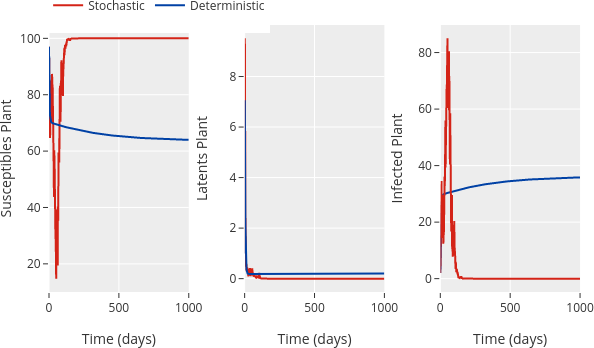
\includegraphics[scale=0.45, keepaspectratio]{%
	Figures/ExtinctionNoise.png}
	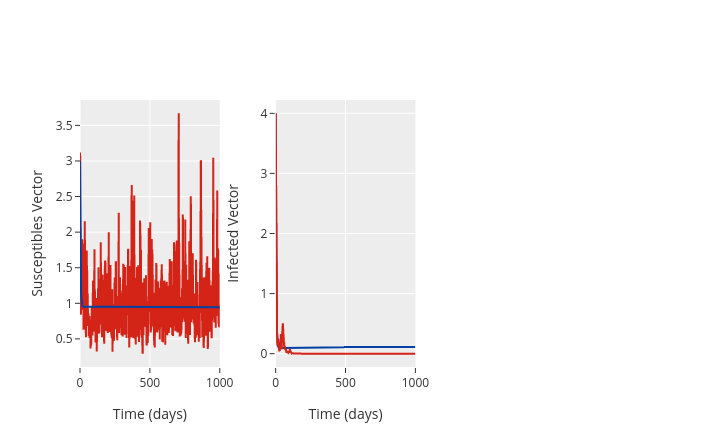
\includegraphics[scale=0.45, keepaspectratio]{%
	Figures/ExtinctionNoiseVector.png}
	\end{center}
	\caption{%
		\href{https://plotly.com/~AdrianSalcedo/2/}{%
		https://plotly.com/~AdrianSalcedo/2/}}
	\label{fig:ExtinctionByNoise}
\end{figure}
\begin{figure}[ht]
	\centering
	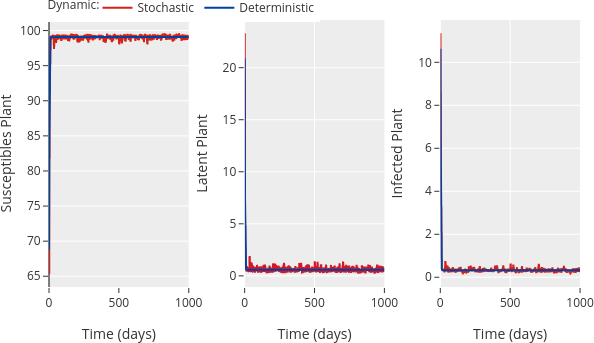
\includegraphics[scale=0.45, keepaspectratio]{%
	Figures/Rs0LessThanOne.png}
	
	\caption{Here we present the $\mathcal{R}^s_0<1$ only plant population}
	\label{fig:Rs0SmallerThanOne}
\end{figure}
\info{Include infected vector dynamics}
\begin{figure}[ht]
	\centering
	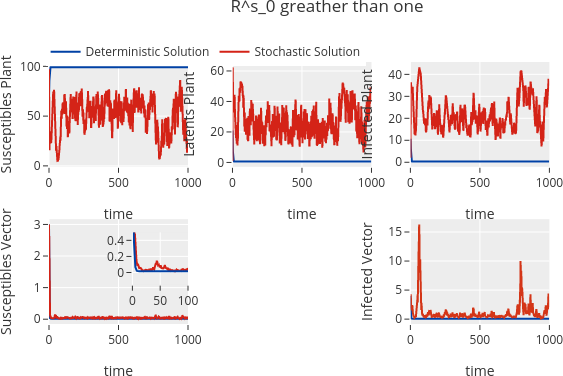
\includegraphics[scale=0.5, keepaspectratio]{%
	Figures/R0_more/R^s_0greather_than_one.png}
	\caption{Caption two}
	\label{fig:Rs0GreatherThanOne}
\end{figure}

\info{Make GitHub repository and bib reference}
\change{Enumerate plot panels}
	\section{Conclusion}
		\label{sec:conclusion}
	% %!TEX root = ./main.tex
%
\pagebreak
\begin{table}
	\begin{tabular}{rcl} 
		\toprule
			Referecnce
			&
			Priority
			&
			Observation
		\\
		\midrule
		\\
		\cite{Zhao2013}
		\\
		\cite{Zhang2017a}	&	**  & See Lyapnov Function.
		\\
		\cite{Liu2018a} &       **  & For persistece def
		\\
		\cite{Liu2018d} &        *   & Dengue
		\\
		\cite{Cai2017a} &        *   & Mobility	
		\\
		\cite{Lu2009} & 
		\\
		\cite{ElFatini2018}
		\\
		\cite{Liu2019b}
		\\
		\cite{Lahrouz2017a}
		\\
		\cite{Wang2018a}
		\\
		\cite{Cao2016a} 	& *** & Review
		\\
		\cite{Tang2015} 	& *** & Review
		\\
		\cite{Ji2014} 		& ** &Review
		\\
		\cite{Liu2018b} 	& * & Vaccination
		\\
		\cite{Cai2015} 		& ** & General ideas
		\\
		\cite{Zhang2018a} 	& *** & For extinction by noise
		\\
		\cite{Zhao2014} 	& *** & Threshold behaviour
		\\
		\cite{Chang2017}    & *** & Good idea for COVID 19
		\\		
		\cite{Dieu2018}     & ** & Lie approach		
		\\
		\cite{Lin2014a}     & **  & Threshold
		\\
		\cite{Maliyoni2017} & ***  	&	 Thickbone with CMCM deduction
		\\
		\cite{Qiu2013}		& ***   &	 Permanence
		\\
		\cite{Lin2017a}		&	*   &	Degenerate Difussion
		\\
		\cite{Cai2013}		&	*   &	General force of infection 
		\\
		\bottomrule
	\end{tabular}
\end{table}
\bibliography{References.bib}{}
\bibliographystyle{spphys}
	\appendix
	\section{Background}
	\info{add a tex source with the appendix files}
\end{document}
